% cd /storage/emulated/0/Documents/documents/latex/1920/Grade-10/2nd/circles-and-related-terms && pdflatex hand-circles-and-related-terms.tex && termux-open hand-circles-and-related-terms.pdf


\documentclass[handout]{beamer} 

\usepackage{pgfpages} 
\mode<handout>{%
\pgfpagesuselayout{4 on 1}[
%letterpaper, 
legalpaper, %landscape, 
border shrink=1mm] 
%\setbeameroption{show notes} 
}

\usepackage{xcolor}
\usepackage{anyfontsize}
\usepackage{enumitem}
\usepackage{multicol}
\usepackage{amsmath}
%\usepackage{amsfonts,dsfont}% for \mathds 
\usepackage{tabularx, booktabs, makecell} 
\usepackage{gensymb}
\usepackage{multirow}
\usepackage{graphicx, tipa}
\usepackage{tikz}
\usetikzlibrary{angles,quotes}
\usepackage{pgfplots} 
\usetikzlibrary{calc}
\pgfplotsset{compat=newest}
\usetikzlibrary{arrows.meta}
\usetikzlibrary{intersections}
\usetikzlibrary{decorations.pathreplacing}
\usepackage{flafter}
\usepackage{amsmath,amssymb,cancel,units}
\usepackage{microtype} % nicer output 
\usepackage{hfoldsty} % nicer output 
\usepackage{fixltx2e} 
\usepackage{mathptmx}
%\usepackage{mnsymbol}
\usepackage{numprint}
\usepackage[utf8]{inputenc} 
\usepackage[T1]{fontenc}

\pagenumbering{gobble}
%\linespread{0.9}
\newcommand{\vspce}{\vspace{0.75ex}}
\newcommand{\hspce}{\hspace{0.5em}}

\newcommand{\vertadjust}{\vspace*{-2.5in}} % legalpaper
%\newcommand{\vertadjust}{\vspace*{-1.5in}} % letterpaper

\newcommand{\blank}{\underline{\hspace{2em}}}%{\rule{1em}{0.15ex}}
\newcommand{\arc}[1]{{% 
\setbox9=\hbox{#1}% 
\ooalign{\resizebox{\wd9}{\height}{\texttoptiebar{\phantom{A}}}\cr#1}}}

\newcolumntype{C}{ >{\centering\arraybackslash} X}

%\frame[shrink=5] 
\begin{document} 
\vertadjust
\begin{frame} %1
\begin{center}
\textbf{Circles and Related Terms}
\end{center}

\vspace*{1ex}

 
\input{ps-circles-and-related-terms-input1}
\vspace*{1.5ex}
B. In $\bigodot V$, $\overline{OL} $ and $\overline{CS} $ are diameters. If $m \angle{AVL}=90 \degree$ and $m \angle{SVL}=40 \degree$, find: 
\begin{enumerate}[label = \arabic*. ]
%begin{multicols}{3}
%1
\item \hspce m\arc{OC}
%2
\item \hspce m\arc{AL}
%3
\item \hspce m\arc{LS}
%4
\item \hspce $m \angle{CVA} $
%5
\item \hspce m\arc{CA}
%6
\item \hspce $m \angle{OVS} $
%7
\item \hspce m\arc{OS}
%8
\item \hspce m\arc{CAS}
%9
\item \hspce $m \angle{AVS} $

\end{multicols} 
\end{enumerate}  

%%\vspace*{10cm}\hspace*{7cm}
\begin{tikzpicture}[dot/.style={circle, fill=black, inner sep=0pt, outer sep=0pt, minimum size=3pt}, dim-label/.style={fill=white, rectangle, inner sep=2pt, outer sep=0pt}, remember picture, overlay, 
nodot/.style={circle, fill=black, inner sep=0pt, outer sep=0pt, minimum size=0pt}
]  


\def\rad1{1cm}


\node(v)[dot] at (0,0) {};
\node(v-label) at ($(v)+(180:7pt)$) {$V$};

\draw[name path=circ, line width=0.5mm] (v) circle (\rad1); 

\node (a) at (0:\rad1) [nodot] {}; 
\node(a-label) at ($(a)+(0:7pt)$) {$A$};

\node (o) at (90:\rad1) [nodot]{}; 
\node(o-label) at ($(o)+(90:7pt)$) {$O$};

\node (l) at (-90:\rad1) [nodot]{}; 
\node(l-label) at ($(l)+(-90:7pt)$) {$L$}; 

\node (c) at (65:\rad1) [nodot]{}; 
\node(c-label) at ($(c)+(65:7pt)$) {$C$}; 

\node (s) at (245:\rad1) [nodot]{}; 
\node(s-label) at ($(s)+(245:7pt)$) {$S$}; 

\draw[line width=0.3mm] (o) -- (l) (c) -- (s) (a) -- (v);  

\end{tikzpicture}
%\vspace*{-3cm}\hspace*{-5cm}    
\vspace*{-1.5ex}
%\input{ps-circles-and-related-terms-input3}
\end{frame}

\vertadjust
\begin{frame} %2
%\begin{center}
\textbf{Circles and Related Terms}
\end{center}

\vspace*{1ex}

 
%\input{ps-circles-and-related-terms-input1}
%\vspace*{1.5ex}
B. In $\bigodot V$, $\overline{OL} $ and $\overline{CS} $ are diameters. If $m \angle{AVL}=90 \degree$ and $m \angle{SVL}=40 \degree$, find: 
\begin{enumerate}[label = \arabic*. ]
%begin{multicols}{3}
%1
\item \hspce m\arc{OC}
%2
\item \hspce m\arc{AL}
%3
\item \hspce m\arc{LS}
%4
\item \hspce $m \angle{CVA} $
%5
\item \hspce m\arc{CA}
%6
\item \hspce $m \angle{OVS} $
%7
\item \hspce m\arc{OS}
%8
\item \hspce m\arc{CAS}
%9
\item \hspce $m \angle{AVS} $

\end{multicols} 
\end{enumerate}  

%%\vspace*{10cm}\hspace*{7cm}
\begin{tikzpicture}[dot/.style={circle, fill=black, inner sep=0pt, outer sep=0pt, minimum size=3pt}, dim-label/.style={fill=white, rectangle, inner sep=2pt, outer sep=0pt}, remember picture, overlay, 
nodot/.style={circle, fill=black, inner sep=0pt, outer sep=0pt, minimum size=0pt}
]  


\def\rad1{1cm}


\node(v)[dot] at (0,0) {};
\node(v-label) at ($(v)+(180:7pt)$) {$V$};

\draw[name path=circ, line width=0.5mm] (v) circle (\rad1); 

\node (a) at (0:\rad1) [nodot] {}; 
\node(a-label) at ($(a)+(0:7pt)$) {$A$};

\node (o) at (90:\rad1) [nodot]{}; 
\node(o-label) at ($(o)+(90:7pt)$) {$O$};

\node (l) at (-90:\rad1) [nodot]{}; 
\node(l-label) at ($(l)+(-90:7pt)$) {$L$}; 

\node (c) at (65:\rad1) [nodot]{}; 
\node(c-label) at ($(c)+(65:7pt)$) {$C$}; 

\node (s) at (245:\rad1) [nodot]{}; 
\node(s-label) at ($(s)+(245:7pt)$) {$S$}; 

\draw[line width=0.3mm] (o) -- (l) (c) -- (s) (a) -- (v);  

\end{tikzpicture}
%\vspace*{-3cm}\hspace*{-5cm}    
\vspace*{-1.5ex}
\input{ps-circles-and-related-terms-input3}
\end{frame}

%\vspace*{-2.7in} %legalpaper
\vertadjust
\begin{frame} %3
\begin{center}
\textbf{Circles and Related Terms}
\end{center}

\vspace*{1ex}

 
\input{ps-circles-and-related-terms-input1}
\vspace*{1.5ex}
B. In $\bigodot V$, $\overline{OL} $ and $\overline{CS} $ are diameters. If $m \angle{AVL}=90 \degree$ and $m \angle{SVL}=40 \degree$, find: 
\begin{enumerate}[label = \arabic*. ]
%begin{multicols}{3}
%1
\item \hspce m\arc{OC}
%2
\item \hspce m\arc{AL}
%3
\item \hspce m\arc{LS}
%4
\item \hspce $m \angle{CVA} $
%5
\item \hspce m\arc{CA}
%6
\item \hspce $m \angle{OVS} $
%7
\item \hspce m\arc{OS}
%8
\item \hspce m\arc{CAS}
%9
\item \hspce $m \angle{AVS} $

\end{multicols} 
\end{enumerate}  

%%\vspace*{10cm}\hspace*{7cm}
\begin{tikzpicture}[dot/.style={circle, fill=black, inner sep=0pt, outer sep=0pt, minimum size=3pt}, dim-label/.style={fill=white, rectangle, inner sep=2pt, outer sep=0pt}, remember picture, overlay, 
nodot/.style={circle, fill=black, inner sep=0pt, outer sep=0pt, minimum size=0pt}
]  


\def\rad1{1cm}


\node(v)[dot] at (0,0) {};
\node(v-label) at ($(v)+(180:7pt)$) {$V$};

\draw[name path=circ, line width=0.5mm] (v) circle (\rad1); 

\node (a) at (0:\rad1) [nodot] {}; 
\node(a-label) at ($(a)+(0:7pt)$) {$A$};

\node (o) at (90:\rad1) [nodot]{}; 
\node(o-label) at ($(o)+(90:7pt)$) {$O$};

\node (l) at (-90:\rad1) [nodot]{}; 
\node(l-label) at ($(l)+(-90:7pt)$) {$L$}; 

\node (c) at (65:\rad1) [nodot]{}; 
\node(c-label) at ($(c)+(65:7pt)$) {$C$}; 

\node (s) at (245:\rad1) [nodot]{}; 
\node(s-label) at ($(s)+(245:7pt)$) {$S$}; 

\draw[line width=0.3mm] (o) -- (l) (c) -- (s) (a) -- (v);  

\end{tikzpicture}
%\vspace*{-3cm}\hspace*{-5cm}    
\vspace*{-1.5ex}
%\input{ps-circles-and-related-terms-input3}
\end{frame}

%\vspace*{-2.7in} %legalpaper
\vertadjust
\begin{frame} %4
%\begin{center}
\textbf{Circles and Related Terms}
\end{center}

\vspace*{1ex}

 
%\input{ps-circles-and-related-terms-input1}
%\vspace*{1.5ex}
B. In $\bigodot V$, $\overline{OL} $ and $\overline{CS} $ are diameters. If $m \angle{AVL}=90 \degree$ and $m \angle{SVL}=40 \degree$, find: 
\begin{enumerate}[label = \arabic*. ]
%begin{multicols}{3}
%1
\item \hspce m\arc{OC}
%2
\item \hspce m\arc{AL}
%3
\item \hspce m\arc{LS}
%4
\item \hspce $m \angle{CVA} $
%5
\item \hspce m\arc{CA}
%6
\item \hspce $m \angle{OVS} $
%7
\item \hspce m\arc{OS}
%8
\item \hspce m\arc{CAS}
%9
\item \hspce $m \angle{AVS} $

\end{multicols} 
\end{enumerate}  

%%\vspace*{10cm}\hspace*{7cm}
\begin{tikzpicture}[dot/.style={circle, fill=black, inner sep=0pt, outer sep=0pt, minimum size=3pt}, dim-label/.style={fill=white, rectangle, inner sep=2pt, outer sep=0pt}, remember picture, overlay, 
nodot/.style={circle, fill=black, inner sep=0pt, outer sep=0pt, minimum size=0pt}
]  


\def\rad1{1cm}


\node(v)[dot] at (0,0) {};
\node(v-label) at ($(v)+(180:7pt)$) {$V$};

\draw[name path=circ, line width=0.5mm] (v) circle (\rad1); 

\node (a) at (0:\rad1) [nodot] {}; 
\node(a-label) at ($(a)+(0:7pt)$) {$A$};

\node (o) at (90:\rad1) [nodot]{}; 
\node(o-label) at ($(o)+(90:7pt)$) {$O$};

\node (l) at (-90:\rad1) [nodot]{}; 
\node(l-label) at ($(l)+(-90:7pt)$) {$L$}; 

\node (c) at (65:\rad1) [nodot]{}; 
\node(c-label) at ($(c)+(65:7pt)$) {$C$}; 

\node (s) at (245:\rad1) [nodot]{}; 
\node(s-label) at ($(s)+(245:7pt)$) {$S$}; 

\draw[line width=0.3mm] (o) -- (l) (c) -- (s) (a) -- (v);  

\end{tikzpicture}
%\vspace*{-3cm}\hspace*{-5cm}    
\vspace*{-1.5ex}
\input{ps-circles-and-related-terms-input3}
\end{frame}

\end{document}

